\documentclass[12pt,a4paper]{article}
\usepackage[utf8]{inputenc}
\usepackage{amsmath}
\usepackage{amsfonts}
\usepackage{amssymb}

%bold Greek letters and other symbols
\usepackage{bm}

\usepackage[T1]{fontenc}
\usepackage[english]{babel}
\usepackage{graphicx}
\usepackage[left=2.5cm,right=2.5cm,top=2.5cm,bottom=2cm]{geometry}
\usepackage{color}
%
\usepackage{makeidx}
\usepackage{shortvrb,latexsym}

\setlength{\parindent}{0pt}
%\renewcommand{\floatpagefraction}{.99}
%\renewcommand{\textfraction}{.01}

\newcommand{\bu}{{\bf u}}
\newcommand{\bv}{{\bf u}}
\newcommand{\rd}{\mathrm{d}}
\newcommand{\hx}{{\bf\hat{x}}}
\newcommand{\hy}{{\bf\hat{y}}}
\newcommand{\hz}{{\bf\hat{z}}}
\newcommand{\hr}{{\bf\hat{r}}}
\newcommand{\hn}{{\bf\hat{n}}}

\begin{document}

\begin{center}
2019-01-16
\end{center}
STOCKHOLMS UNIVERSITET\\
Meteorologiska Institutionen\\
Jonas Nycander, Dhrubaditya Mitra\\
\vspace{1cm}

\begin{center}
{\bf\large Exam in Fluid mechanics (MO5001)}\\
\end{center}

Write the solution of each problem on a separate paper, and write your identification number on every paper.\\

{\bf Allowed aids:} calculator, sheet with vector analysis relations.\\

{\bf Grading:} A 90-100\%, B 80-89\%, C 65-79\%, D 55-64\%, E 50-54\%, Fx 45-49\%, F 0-44\% \\
\vspace{0.5cm}

\begin{enumerate}
  %====================================================================
\item \label{prb1} Answer the following short questions. You just need to write the final answer. Each question is worth 2 points. 
  \begin{enumerate}
  \item A scalar function of three Cartesian coordinates, $x,y,z$ is 
    \begin{equation}
       T(x,y,z) = \sin(x)\cos(y) + \cos(y)\sin(z)
    \end{equation}
    If $\vec{G} = \vec{\nabla} T $ then calculate $\vec{\nabla}\times \vec{G}$.
  \item After deformation the displacement field in a material is given by the following expression
    \begin{eqnarray}
      u_x = \alpha [2x + \sin(y) + 5z^3 ] \\
      u_y = \alpha[ e^{-x} - y + \cos(z) ] \\
      u_z = \alpha[ \sin(x) + \cos(y) -z ]
    \end{eqnarray}
    Here $\alpha$ is small such that you can apply the approximation of small deformation everywhere. 
    Under this deformation calculate the change is volume of the material.
  \item In which of the following cases can I write the velocity $\vec{v} = \nabla \Psi $ where $\Psi$ is a scalar function
    without any loss of generality: \\
    (a) if the flow is incompressible, (b) if the flow is irrotational, or (c) if the flow is steady.
  \item In a turbulent boundary layer very close to the wall how does the mean stream-wise
    velocity ($\langle v_x \rangle$) depends on the wall-normal coordinate ($y$) ? 
  \item The lubrication approximation, equations that describes a laminar boundary layer, and the
    shallow-water equations are all derived
    from the incompressible Navier--Stokes equations. 
    They all assume  that the Reynolds number is small. 
    What is another crucial common aspect of all these derivations  ?  
    \end{enumerate}

\item \label{prb2} Two manometric tubes are mounted on a horizontal pipe of varying
  cross-section
  at the sections $S_1$ and $S_2$ (see left panel of figure~\ref{pipe_disc}).
  Find the flux ( volume of water flowing across the pipe's cross section per unit time )
  if the difference in water columns is equal to $\Delta h$.
  (5 p)
\item \label{prb3} A thin rectangular plate of dimension $L_x\times L_z$ 
is immersed in a fluid  of
kinematic viscosity $\nu$ and density $\rho$. The plate is being
pulled by a force such that it moves with a velocity $v$ along the $x$
direction. Far away from the plate the fluid is at rest. Assume that the flow is
  laminar. Ignore the edge effects. 
  Estimate the the power necessary to keep the plate moving with a constant velocity.
    (Hint : The power necessary
    is equal to the power dissipated by the viscous forces. You can estimate the
    viscous forces from the stress at the surface of the disc. You need the thickness
    of the boundary layer to estimate the stress. ) (5p)

\item \label{prb4} Same as in Problem~\ref{prb3} with an additional feature:
  the plate is confined vertically within a cavity. The clearance between the
  disk and the horizontal planes of the cavity is equal to $h$ where $h \ll L_x $
   as shown in figure~\ref{pipe_disc}.
   Ignore the edge effects. 
  Calculate  the the power necessary to keep the plate moving. 
    (Hint : Use lubrication approximation )  (5p)

  \begin{figure}
    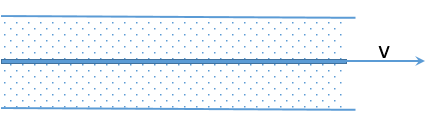
\includegraphics[width=0.5\linewidth]{plate.png}
    \caption{\label{pipe_disc} Problem \ref{prb4} }
  \end{figure}

%===================================================

\item 
The horizontal component of the momentum equation for a fluid in a rotating
system is
$$
\frac{\partial\bu}{\partial t}+\bu\cdot\nabla\bu+f\hz\times\bu =
-\frac{\nabla_z p}{\rho}+\nu\nabla^2 \bu,
$$
where $\nabla_z$ denotes the horizontal components of $\nabla$. We assume the velocity $\bu(x,y.z,t)$ to be purely horizontal, and the density $\rho$ to be constant.
\begin{enumerate}
  \item Define the Rossby number and the Ekman number in terms of the time
  scale $T$, horizontal length scale $L$, vertical length scale $H$, and the
  coefficients of the equation, and explain how these numbers measure the ratio between
  various terms in the equation above.
  \item Assume that the Rossby number and the Ekman number are both small, and derive
  an approximate expression for $\bu$.
  \item Assume that there is a solid boundary at $z=0$, with fluid above it, and that $\bu$ is
  stationary and horizontally homogeneous, i.e.\ does not depend on $t, x$ or $y$. Simplify
  the equation above for this case, and give the appropriate boundary condition at $z=0$.
  \item Assume that the flow is constant far above the boundary, i.e.\ $\bu=u_0\hx $,
  where $u_0=const.$ This flow does not satisfy the boundary condition at $z=0$. 
  Explain how the boundary condition can be satisfied. Also estimate the thickness of the
  layer in which the flow is not constant, by estimating the the magnitude of the terms in the
  equation obtained in (c). It is not necessary to solve the equation.
 \end{enumerate}

(10 p) \\
%====================================================================
\item
The non-rotating shallow-water equations are
$$
\frac{\partial \bu}{\partial t}+\bu\cdot\nabla\bu = -g\nabla h,
$$
$$
\frac{\partial h}{\partial t}+\nabla\cdot(\bu h) = 0,
$$
where $h$ is the depth and $\bu$ the velocity.
\begin{enumerate}
  \item Linearise the equations around a suitable background state.
  \item Derive the dispersion relation for linear waves.
  \item How long time does it take for a wave of this kind to cross the Atlantic? Assume
  that it is 4000 km wide and 4000 m deep.
\end{enumerate}

(10 p)\\
%====================================================================
\item
The rotating shallow-water equations are
$$
\frac{\partial \bu}{\partial t}+\bu\cdot\nabla\bu+f\hz\times\bu
= -g\nabla h,
$$
$$
\frac{\partial h}{\partial t}+\nabla\cdot(\bu h) = 0,
$$
where $h$ is the depth and $\bu$ the velocity. Assume that the water is 
surrounded by a solid boundary (a coast). Specify suitable boundary conditions, 
and show that the total mass is conserved.

(5 p)\\
%====================================================================
\end{enumerate}
\end{document}
